\chapter{Architecture}
\label{chapter4}


In the section, we will provide detailed description of the architecture of neural networks for automatic GEC task. The architecture consists of a bidirectional RNN as an encoder and a decoder that emulates searching through a source sentence during decoding a correction. The architecture of the neural network model we built is shown in the following figure.

\begin{figure}[ht]
    \centering
    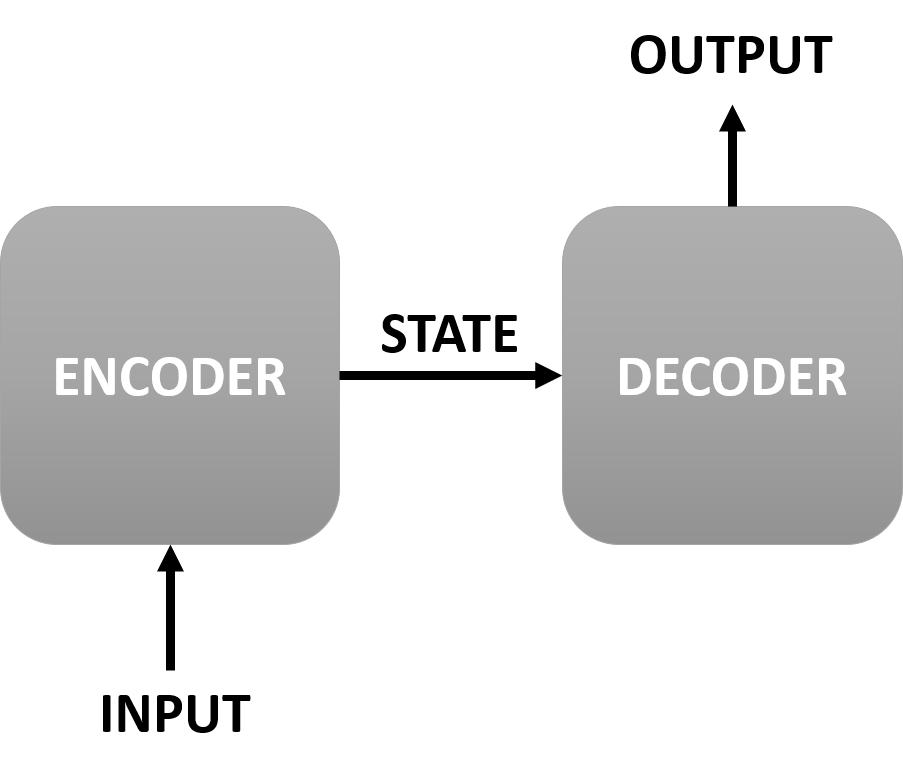
\includegraphics[width=0.8\textwidth]{EDA.png}
    \caption{Encoder and Decoder Structure.}
    \label{fig:5}
\end{figure}

\section{Decoder}

As the illustration in Section 3, the encoder is to read the input sentence, a sequence of vectors $\mathbf{x}=\left(x_1,\ldots,x_T\right)$, and convert the input sentence into a vector $c$. As the encoder reads each symbol, the hidden state of the RNN for each step, saying $h$, changes as the equations shown in the last section.

In this model architecture, we define each conditional probability as:
$$p\left(y_i\middle|\left\{y_{i-1},\ldots,y_1\right\},\mathbf{x}\right)=g\left(y_{i-1},s_i,c_i\right),$$
where $s_i$ is an RNN hidden state for time $i$, computed by
$$s_i=f\left(s_{i-1},y_{i-1},c_i\right).$$
Please note that the approach here is different from the traditional encoder–decoder approach. Here, the probability is conditioned on a distinct context vector $c_i$ for each target word $y_i$ while the traditional one is conditioned on the sequence.

The context vector $c_i$ depends on a sequence of annotation $\left\{h_1,\ldots,h_T\right\}$ to which an encoder maps the input sentence. Each annotation $h_i$ contains information about the whole input sequence with a strong focus on the parts surrounding the $i$-th word of the input sequence.

The context vector $c_i$ is, then, computed as a weighted sum of these annotations $h_i$:
$$c_i=\sum_{j=1}^{T}\alpha_{ij}h_j.$$
The weight $\alpha_{ij}$ of each annotation $h_j$ is computed by
$$\alpha_{ij}=\frac{\exp\left(e_{ij}\right)}{\sum_{k=1}^{T}\exp\left(e_{ik}\right)},$$
where 
$$e_{ij}=a\left(s_{i-1},h_j\right).$$
is an alignment model which scores how well the inputs around position $j$ and the output at position $i$ match. The score is based on the RNN hidden state $s_{i-1}$  and $j$-th annotation $h_j$ of the input sentence.

We parametrize the alignment model as a feedforward neural network which is jointly trained with all the other components of the proposed system. Note that unlike in traditional machine translation, the alignment is not considered to be a latent variable. Instead, the alignment model directly computes a soft alignment, which allows the gradient of the cost function to be backpropagated through. This gradient can be used to train the alignment model as well as the whole translation model jointly. 

We can understand the approach of taking a weighted sum of all the annotations as computing an expected annotation, where the expectation is over possible alignments. Let $\alpha_{ij}$ be a probability that the target word $y_i$ is aligned to, or corrected from, a source word $x_j$. Then, the $i$-th context vector $c_i$ is the expected annotation over all the annotations with probabilities $\alpha_{ij}$.

The probability $\alpha_{ij} $, or its associated energy $e_{ij}$, reflects the importance of the annotation $h_j$ with respect to the previous hidden state $s_{i-1}$ in deciding the next state $s_i$ and generating $y_i$. Intuitively, this implements a mechanism of attention in the decoder. The decoder decides parts of the source sentence to pay attention to. By letting the decoder have an attention mechanism, we relieve the encoder from the burden of having to encode all information in the source sentence into a fixed length vector. With this new approach the information can be spread throughout the sequence of annotations, which can be selectively retrieved by the decoder accordingly.

\begin{figure}[ht]
    \centering
    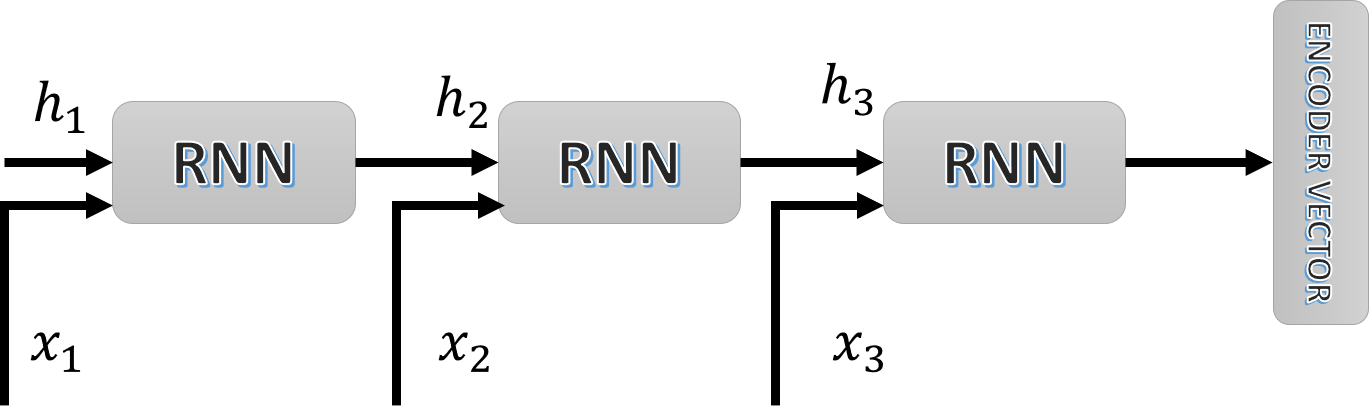
\includegraphics[width=0.8\textwidth]{ECODER.png}
    \caption{Structure of Encoder.}
    \label{fig:6}
\end{figure}

\section{Encoder}
The usual RNN reads an input sequence $\mathbf{x}$ in order starting from the first symbol $x_1$ to the last one $x_T$ . However, in the proposed scheme, we would like the annotation of each word to summarize not only the preceding words, but also the following words. Hence, we use a bidirectional RNN \cite{schuster1997bidirectional}.

A BiRNN consists of forward and backward RNN’s. The forward RNN $\vec{f}$ reads the input sequence  as it is ordered and calculates a sequence of forward hidden states $\left({\vec{h}}_1,\ldots,{\vec{h}}_T\right)$. 
The backward RNN $f$ reads the sequence in the reverse order (from $x_T$ to $x_1$), resulting in a sequence of backward hidden states $\vec{h}_1,\ldots,{\vec{h}}_T$. 
We obtain an annotation for each word $x_j$ by concatenating the forward hidden state ${\vec{h}}_j$ and the backward one ${\bar{h}}_j$ , i.e., $h_j=[\vec{h}_j^T;\bar{h}_T^T]T$. 
In this way, the annotation $h_j$ contains the summaries of both the preceding words and the following words. Due to the tendency of RNNs to better represent recent inputs, the annotation $h_j$ will be focused on the words around $x_j$ . This sequence of annotations is used by the decoder and the alignment model later to compute the context vector.

\begin{figure}[ht]
    \centering
    \includegraphics[width=0.8\textwidth]{Decoder.png}
    \caption{Structure of Decoder.}
    \label{fig:7}
\end{figure}